%%%%%%%%%%%%%%%%%%%%%%%%%%%%%%%%%%%%%%%%%
% Beamer Presentation
% LaTeX Template
% Version 1.0 (10/11/12)
%
% This template has been downloaded from:
% http://www.LaTeXTemplates.com
%
% License:
% CC BY-NC-SA 3.0 (http://creativecommons.org/licenses/by-nc-sa/3.0/)
%
%%%%%%%%%%%%%%%%%%%%%%%%%%%%%%%%%%%%%%%%%

%----------------------------------------------------------------------------------------
%	PACKAGES AND THEMES
%----------------------------------------------------------------------------------------

\documentclass{beamer}

\mode<presentation> {
	
	% The Beamer class comes with a number of default slide themes
	% which change the colors and layouts of slides. Below this is a list
	% of all the themes, uncomment each in turn to see what they look like.
	
	%\usetheme{default}
	%\usetheme{AnnArbor}
	%\usetheme{Antibes}
	%\usetheme{Bergen}
	%\usetheme{Berkeley}
	%\usetheme{Berlin}
	%\usetheme{Boadilla}
	%\usetheme{CambridgeUS}
	%\usetheme{Copenhagen}
	%\usetheme{Darmstadt}
	%\usetheme{Dresden}
	%\usetheme{Frankfurt}
	%\usetheme{Goettingen}
	%\usetheme{Hannover}
	%\usetheme{Ilmenau}
	%\usetheme{JuanLesPins}
	%\usetheme{Luebeck}
	\usetheme{Madrid}
	%\usetheme{Malmoe}
	%\usetheme{Marburg}
	%\usetheme{Montpellier}
	%\usetheme{PaloAlto}
	%\usetheme{Pittsburgh}
	%\usetheme{Rochester}
	%\usetheme{Singapore}
	%\usetheme{Szeged}
	%\usetheme{Warsaw}
	
	% As well as themes, the Beamer class has a number of color themes
	% for any slide theme. Uncomment each of these in turn to see how it
	% changes the colors of your current slide theme.
	
	%\usecolortheme{albatross}
	\usecolortheme{beaver}
	%\usecolortheme{beetle}
	%\usecolortheme{crane}
	%\usecolortheme{dolphin}
	%\usecolortheme{dove}
	%\usecolortheme{fly}
	%\usecolortheme{lily}
	%\usecolortheme{orchid}
	%\usecolortheme{rose}
	%\usecolortheme{seagull}
	%\usecolortheme{seahorse}
	%\usecolortheme{whale}
	%\usecolortheme{wolverine}
	
	%\setbeamertemplate{footline} % To remove the footer line in all slides uncomment this line
	%\setbeamertemplate{footline}[page number] % To replace the footer line in all slides with a simple slide count uncomment this line
	
	%\setbeamertemplate{navigation symbols}{} % To remove the navigation symbols from the bottom of all slides uncomment this line
}

\usepackage{graphicx} % Allows including images
\usepackage{subfigure}
\usepackage{booktabs} % Allows the use of \toprule, \midrule and \bottomrule in tables
\usepackage{bm}

%----------------------------------------------------------------------------------------
%	TITLE PAGE
%----------------------------------------------------------------------------------------

\title[SCAD]{SCAD: Smoothly Clipped Absolute Deviation Penalty} 

\author{Ganchao Wei} 
\date{November 3, 2021}

\begin{document}
	
	\begin{frame}
		\titlepage % Print the title page as the first slide
	\end{frame}
	
	\begin{frame}
		\frametitle{Overview} % Table of contents slide, comment this block out to remove it
		\tableofcontents
	\end{frame}
	
	%--------------------------------------------------------------------
	%	PRESENTATION SLIDES
	%--------------------------------------------------------------------
	
	\section{Penalized Least Squares and Variable Selection}
	
	\begin{frame}
		\frametitle{Penalties}
		Consider the linear regression model $\bm{y}=\bm{X\beta} + \bm{\epsilon}$. Denote $\bm{z}=\bm{X}^{T}\bm{y}$ and let $\hat{\bm{y}} = \bm{XX}^T\bm{y}$. Then a form of the penalized least square squares is
		\begin{figure}
			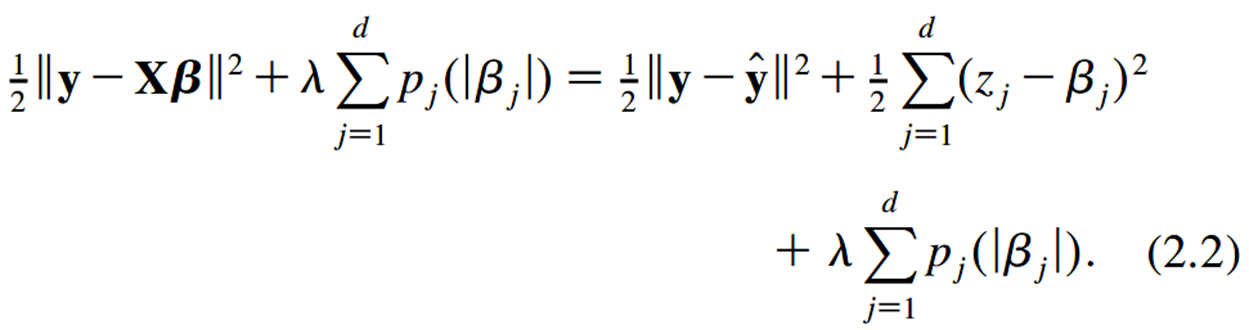
\includegraphics[width=0.8\linewidth]{image001.png}
		\end{figure} 
		Further, denote $p_{\lambda}(|\cdot|) = \lambda p(|\cdot|)$. Minimizing (2.2) leads us to consider the penalized least squares problem
		$$\frac{1}{2}(z-\theta)^2 + p_{\lambda}(|\theta|)$$
	\end{frame}
	
	
	\begin{frame}
		\frametitle{Penalties}
		A good penalty function should have 3 properties:
		\begin{itemize}
			\item
			\textbf{Unbiasedness}: The resulting estimator is nearly unbiased when the true unknown parameter is large to avoid unnecessary modeling bias.
			\item
			\textbf{Sparsity}: The resulting estimator is a thresholding rule, which automatically sets small estimated coefficients to zero to reduce model complexity.
			\item
			\textbf{Continuity}: The resulting estimator is continuous in data $z$ to avoid instability in model prediction.
		\end{itemize}
		What are conditions to satisfy these properties?
	\end{frame} 
	
	
	\begin{frame}
		\frametitle{Penalties}
		First order derivative for $\frac{1}{2}(z-\theta)^2 + p_{\lambda}(|\theta|)$ w.r.t. $\theta$ is $\text{sgn}(\theta)\{|\theta| + p'_{\lambda}(|\theta|)\} - z$
		\begin{itemize}
			\item
			sufficient condition for \textbf{Unbiasedness}: $p'_{\lambda}(|\theta|)=0$ for large $|\theta|$
			\item
			sufficient condition for \textbf{Sparsity}: $min(|\theta| + p'_{\lambda}(|\theta|)) > 0$
			\item
			iff condition for \textbf{Continuity}:$min(|\theta| + p'_{\lambda}(|\theta|))$ is attained at 0
		\end{itemize}
		Let use these criteria to evaluate different penalties: (1) Hard thresholding penalty; (2) $L_q$ penalty $p_{\lambda}(|\theta|) = \lambda |\theta|^q$ (LASSO when $q=1$); (3) SCAD penalty
	\end{frame}
	
	
	\begin{frame}
		\frametitle{Penalties}
		Three penalties \& corresponding thresholding functions.
		\begin{figure}
			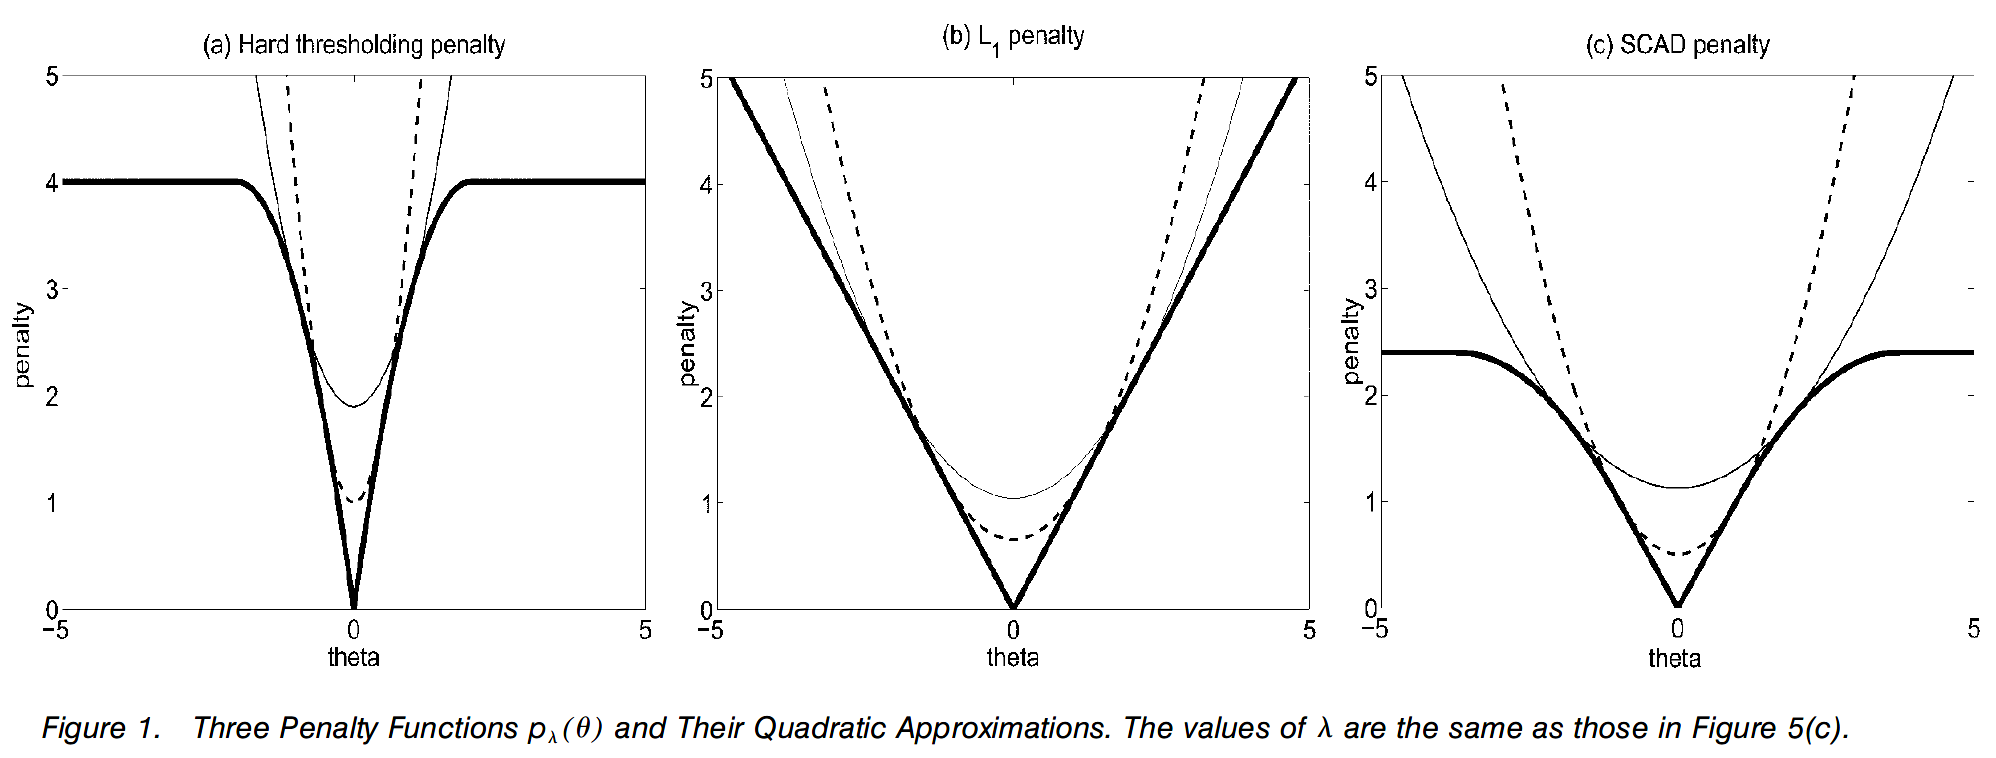
\includegraphics[width=0.7\linewidth]{image002.png}
			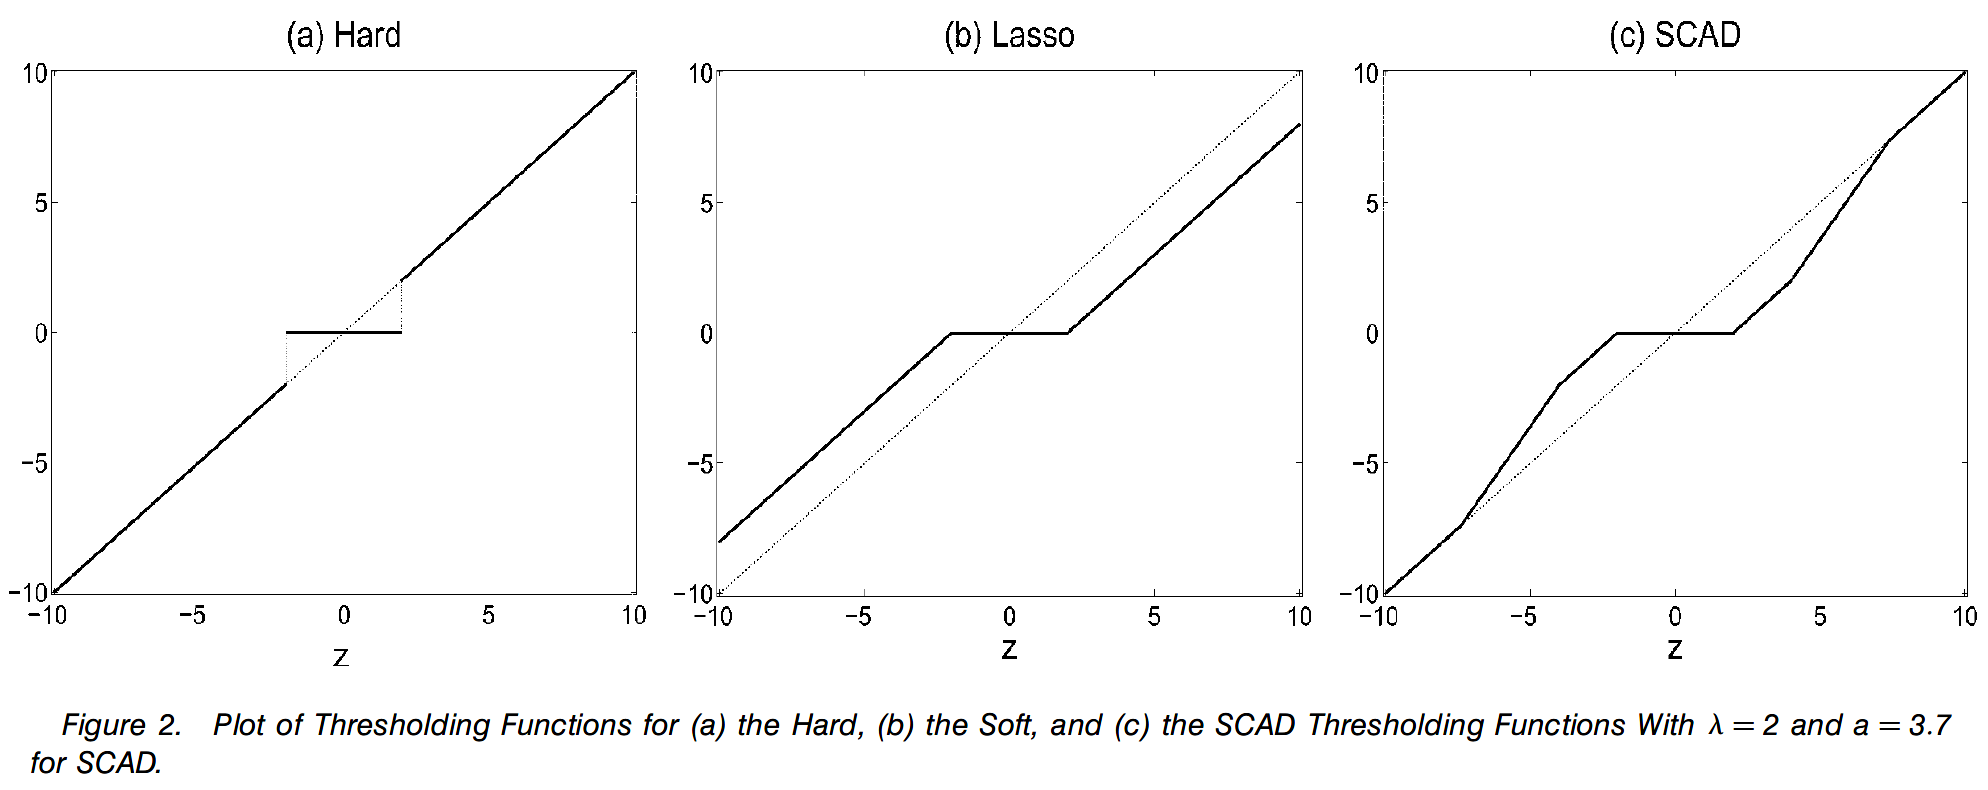
\includegraphics[width=0.7\linewidth]{image003.png}
		\end{figure}
		Hard thresholding: not continuous; LASSO: bias
	\end{frame}
	
	\begin{frame}
		\frametitle{Discussion on $L_q$ penalty}
		Continuous only when $q\geq 1$. But when $q > 1$, $min(|\theta| + p'_{\lambda}(|\theta|)) = 0$
		$\rightarrow$ only when $q = 1$, sparse and continuous
		\begin{figure}
			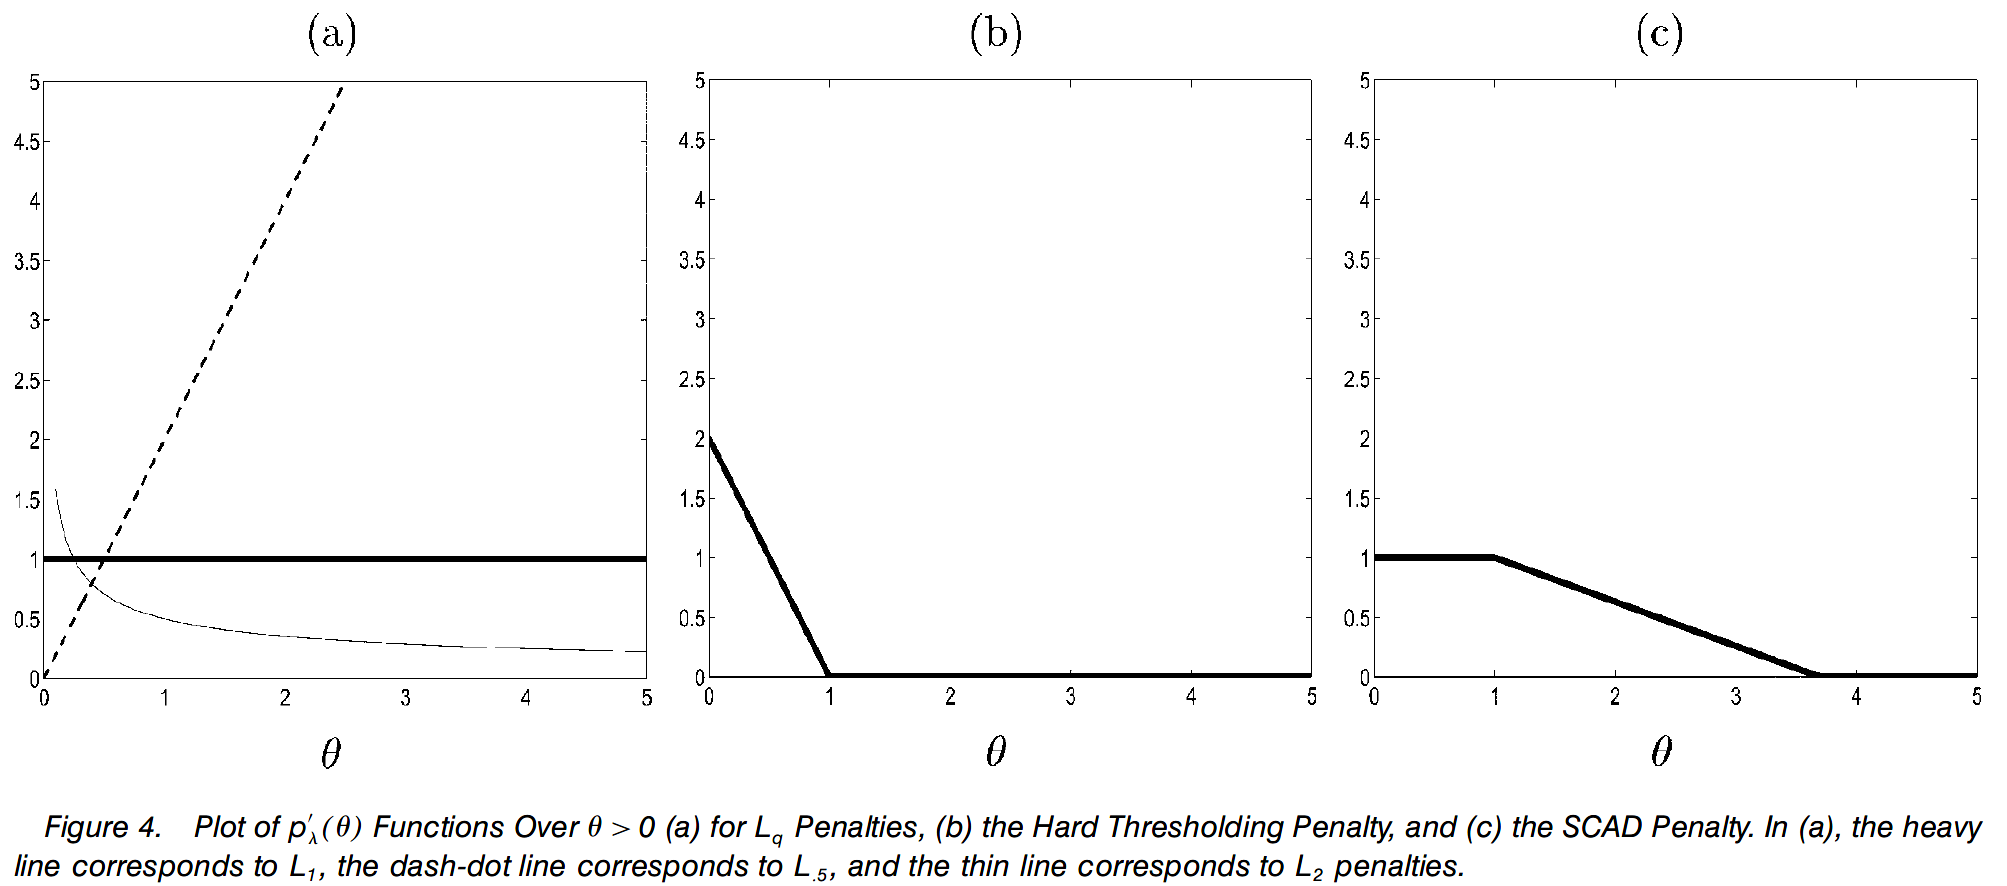
\includegraphics[width=0.8\linewidth]{image005.png}
		\end{figure}
		However, as shown previously, it's bias...
	\end{frame}
	
	\begin{frame}
		\frametitle{Smoothly Clipped Absolute Deviation Penalty}
		The SCAD is defined by the following first order derivative:
		\begin{figure}
			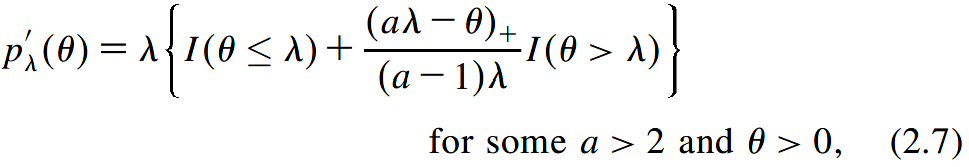
\includegraphics[width=0.7\linewidth]{image007.png}
		\end{figure}
		The resulting solution is given by
		\begin{figure}
			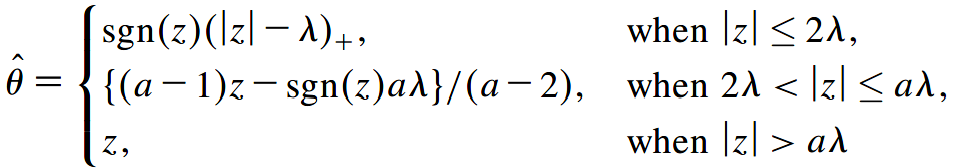
\includegraphics[width=0.7\linewidth]{image008.png}
		\end{figure}
	\end{frame}
	
	\begin{frame}
		\frametitle{Tuning Parameters for SCAD}
		Can be chosen by cross-validation, but computationally expensive. Can implement tools in Bayesian risk analysis. Assume the prior is $\theta \sim N(0, a\lambda)$. Calculate the Bayes risk for $\lambda = \sqrt{2\log(d)}$ for $d = 512, 1024, 2048, 4096$. It seems $a\approx 3.7$ is fine for all cases.
		\begin{figure}
			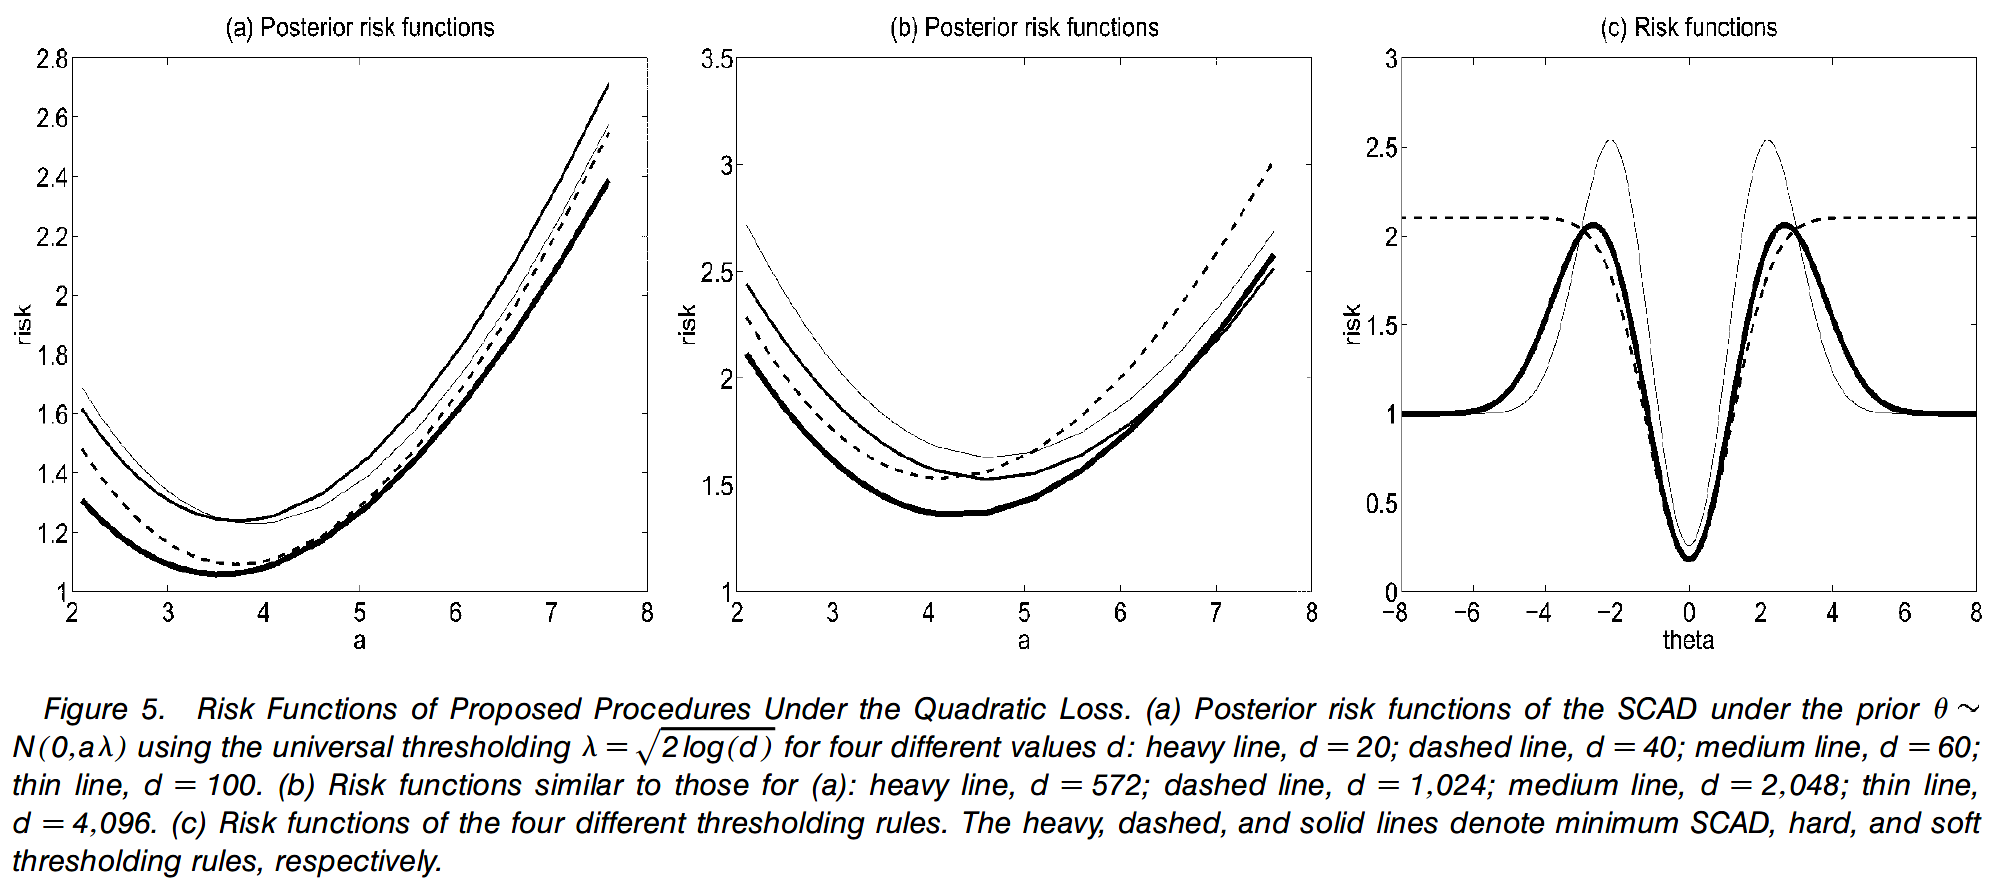
\includegraphics[width=0.9\linewidth]{image006.png}
		\end{figure}
	\end{frame}
	
	\section{Variable Selection via Penalized Likelihood}
	
	\begin{frame}
		\frametitle{Penalized Least Square and Likelihood}
		\begin{itemize}
			\item
			Linear Regression:
			\begin{figure}
				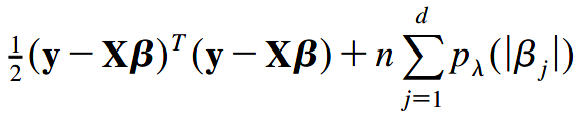
\includegraphics[width=0.5\linewidth]{image009.png}
			\end{figure}
			\item
			Robust Regression:
			\begin{figure}
				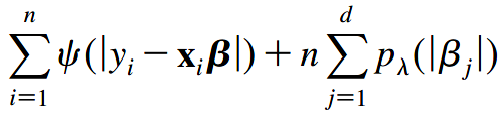
\includegraphics[width=0.5\linewidth]{image010.png}
			\end{figure} 
			\item
			GLM:
			\begin{figure}
				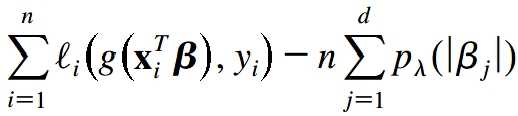
\includegraphics[width=0.5\linewidth]{image011.png}
			\end{figure}  
		\end{itemize}
	\end{frame}
	
	
	\begin{frame}
		\frametitle{Sampling Properties and Oracle Properties}
		Firstly, some notations:
		\begin{itemize}
			\item
			Let $\bm{\beta}_0 = (\bm{\beta}_{10}^T, \bm{\beta}_{20}^T)^T$, where $\bm{\beta}_{20} = \bm{0}$. Let $I(\bm{\beta}_0)$ be Fisher information and let $I(\bm{\beta}_{10}, \bm{0})$ be the Fisher information knowing $\bm{\beta}_{20} = \bm{0}$.
			\item
			Set $\bm{V}_i = (\bm{X}_i, Y_i)$. Let $L(\bm{\beta})$ be the log-likelihood and $Q(\bm{\beta})$ be the penalized likelihood.
		\end{itemize}
		Then we can first show the existence of a penalized likelihood estimator converging at rate $O_p(n^{-1/2} + a_n)$
		\begin{figure}
			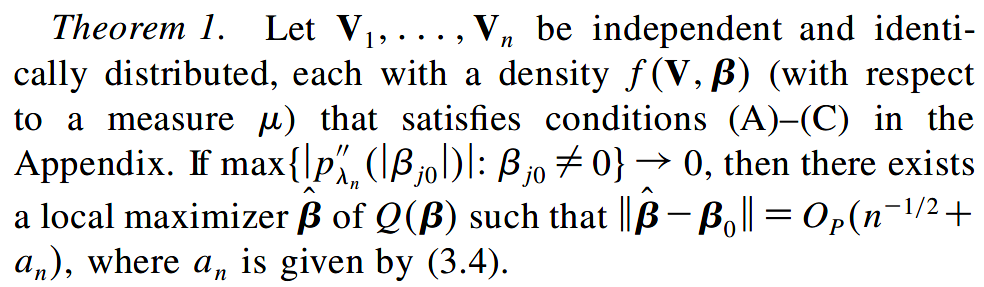
\includegraphics[width=0.8\linewidth]{image012.png}
		\end{figure}
	\end{frame}
	
	
	\begin{frame}
		\frametitle{Sampling Properties and Oracle Properties}
		The oracle property:
		\begin{figure}
			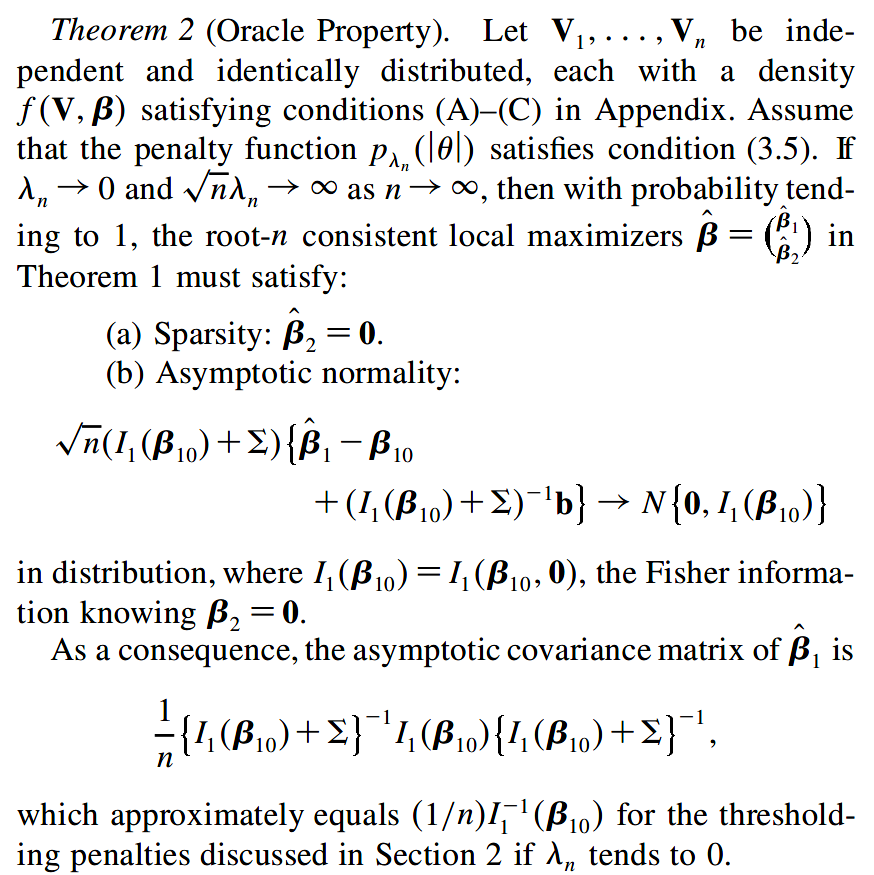
\includegraphics[width=0.6\linewidth]{image013.png}
		\end{figure}
		
	\end{frame}
	
	
	\begin{frame}
		\frametitle{A New Unified Algorithm}
		Use quadratic approximation and update by Newton-Raphson.
		\begin{figure}
			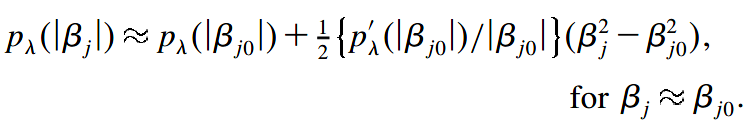
\includegraphics[width=0.6\linewidth]{image014.png}
			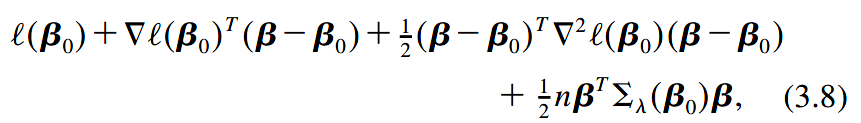
\includegraphics[width=0.6\linewidth]{image015.png}
		\end{figure}
		For linear regression:
		\begin{figure}
			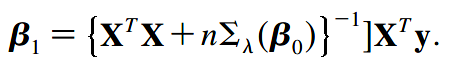
\includegraphics[width=0.3\linewidth]{image016.png}
		\end{figure}
		For robust regression:
		\begin{figure}
			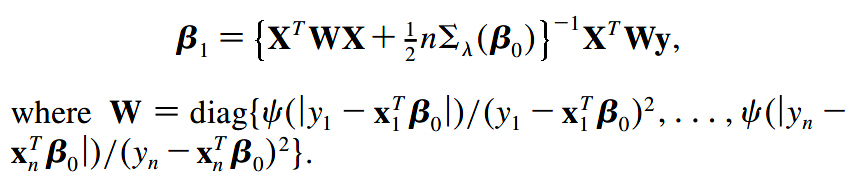
\includegraphics[width=0.6\linewidth]{image017.png}
		\end{figure}
	\end{frame}
	
	
	\begin{frame}
		\frametitle{Standard Error Formula}
		Use sandwich formula.
		\begin{figure}
			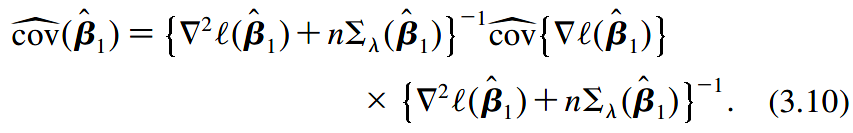
\includegraphics[width=0.7\linewidth]{image018.png}
		\end{figure}
	\end{frame}
	
	\section{Simulation}
	\begin{frame}
		\frametitle{Simulation 1: Linear Regression}
		$Y = \bm{x}^T\bm{\beta} + \sigma\epsilon$
		, where $\bm{\beta} = (3, 1.5, 0, 0, 2 ,0 ,0 ,0)^T$, and the components of $\bm{x}$ and $\epsilon$ are standard normal. The correlation between $x_i$ and $x_j$ is $\rho^{|i-j|}$ with $\rho = .5$.\\
		\vspace{\baselineskip}
		when sample size is small and noise level is high, LASSO is best.\\
		\vspace{\baselineskip}
		when noise level reduce/ sample size increase, SCAD pops out.
	\end{frame}
	
	\begin{frame}
		\frametitle{Simulation 1: Linear Regression}
		\begin{figure}
			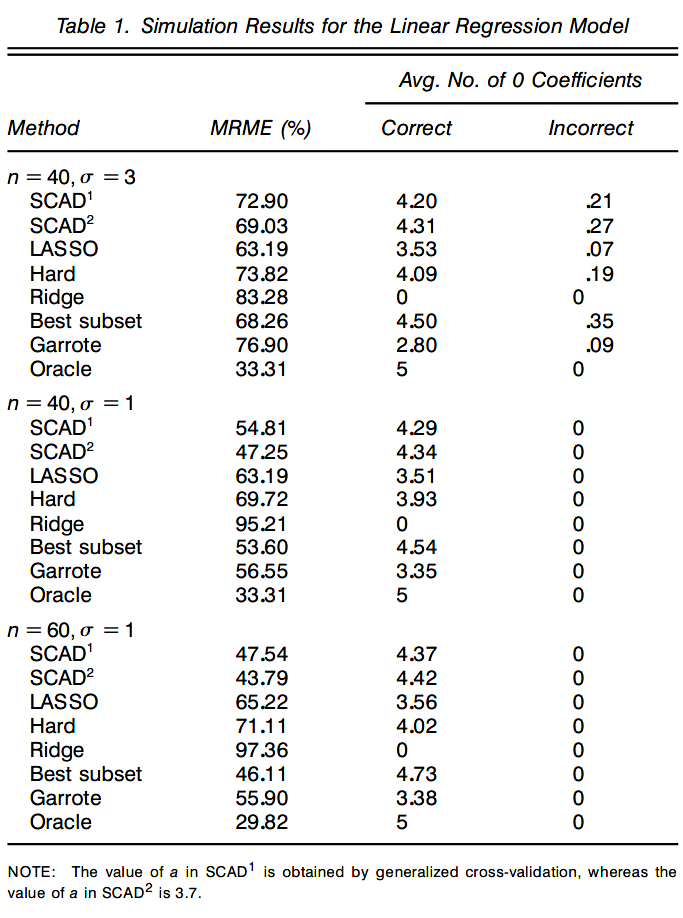
\includegraphics[width=0.5\linewidth]{image019.png}
		\end{figure}
	\end{frame}
	
	\begin{frame}
		\frametitle{Simulation 1: Linear Regression}
		\begin{figure}
			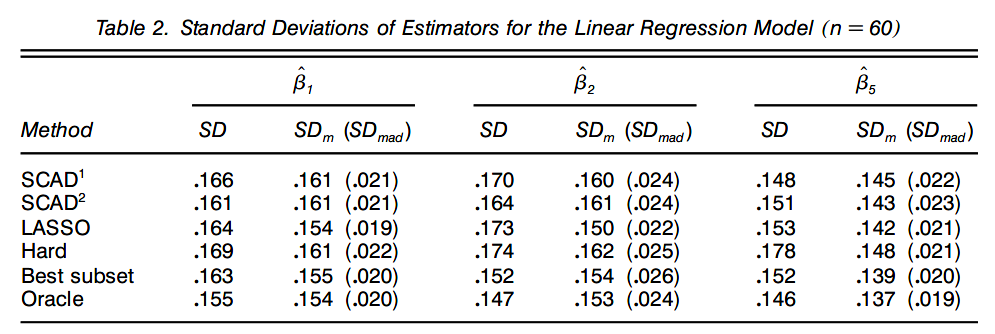
\includegraphics[width=0.9\linewidth]{image020.png}
		\end{figure}
	\end{frame}
	
	\begin{frame}
		\frametitle{Simulation 2: Robust Regression}
		\begin{figure}
			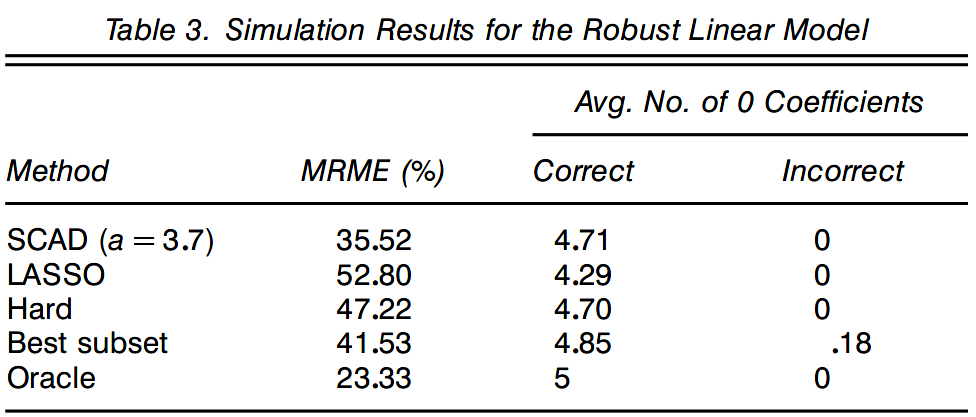
\includegraphics[width=0.6\linewidth]{image021.png}
			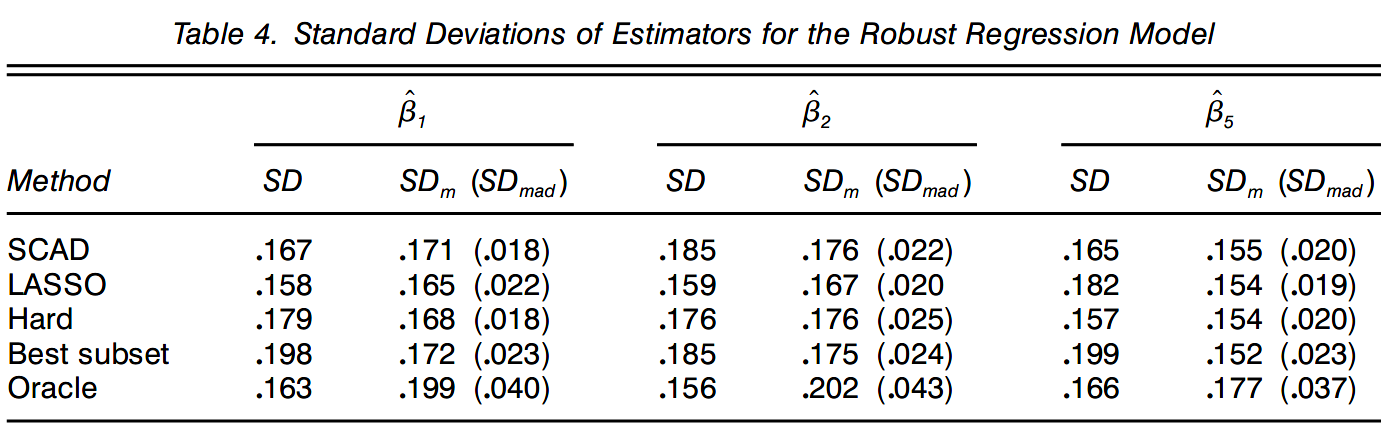
\includegraphics[width=0.9\linewidth]{image022.png}
		\end{figure}
	\end{frame}
	
	\begin{frame}
		\frametitle{Simulation 3: Logistic Regression}
		\begin{figure}
			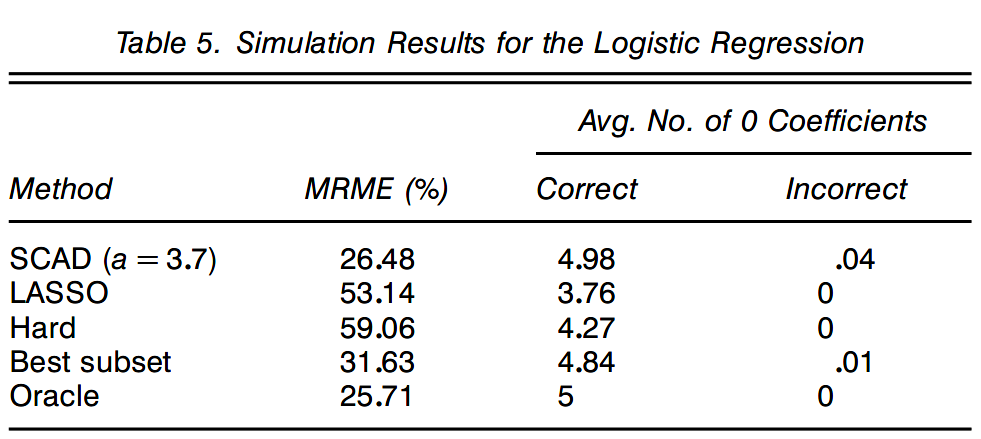
\includegraphics[width=0.6\linewidth]{image023.png}
			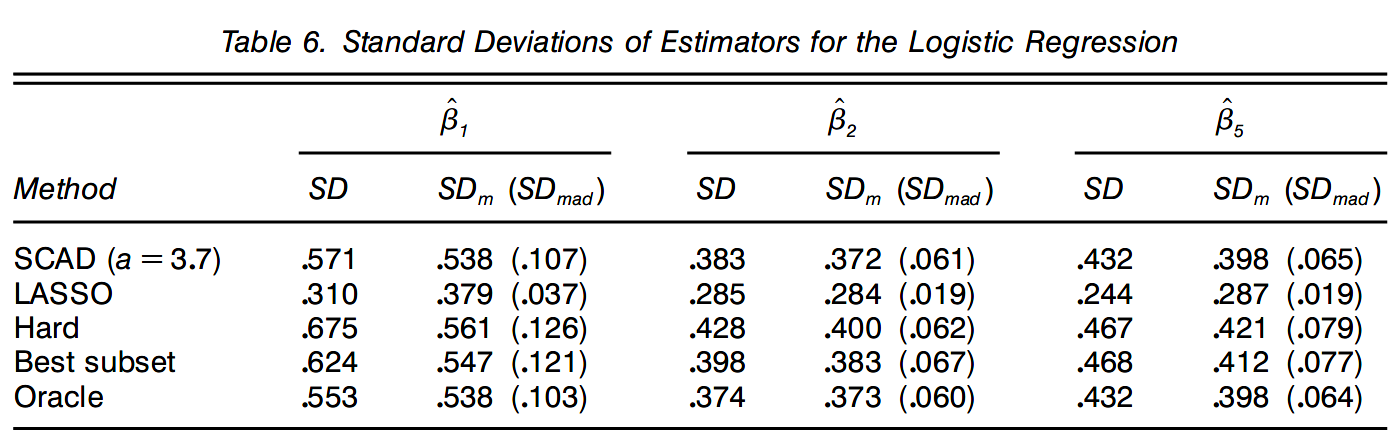
\includegraphics[width=0.9\linewidth]{image024.png}
		\end{figure}
	\end{frame}
	
	\section{Application}
	\begin{frame}
		\frametitle{Burns Data}
		\begin{figure}
			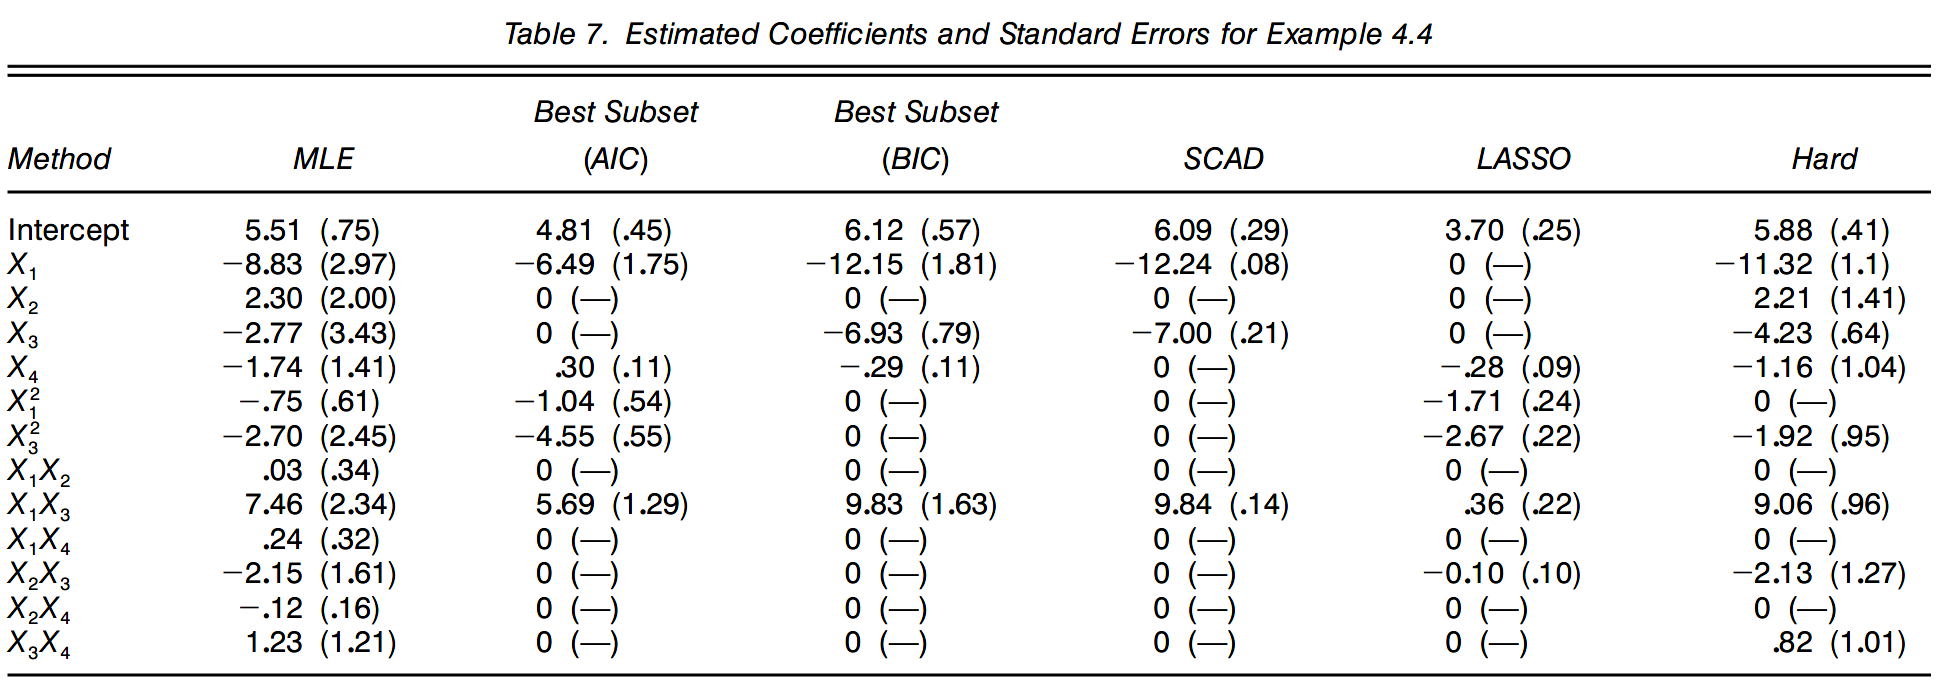
\includegraphics[width=1\linewidth]{image025.png}
		\end{figure}
	\end{frame}
	
	
	
	
\end{document}